\section{Системийн судалгаа}
Сонгосон сэдэв болох ``Ажил олгогчдын өгөгдөлд суурилсан чатбот'' сэдвийн хүрээнд судалгаа хийхдээ чатбот системийн талаар болон өгөгдөл цуглуулгын аргын талаар судалсан. Үүний дараа ижил төстэй системийн болон ашиглагдах технологийн талаар судалгааг хийсэн болно.
\subsection{Чатбот систем}
Чатбот систем нь ихэвчлэн хэрэглэгчийн асуултыг хиймэл оюун ухааны тусламжтайгаар ойлгож, хариултыг автоматжуулах үндсэн зорилготой компьютерийн програм хангамж юм. Орчин үед хэрэглэгчдэд туслах үндсэн үүргийн дагуу чатбот системийг байгууллагууд олон янзаар ашиглах болсон. Тэдгээрээс дурдвал,
\begin{itemize}
  \item Цэс дээр суурилсан чатбот (Menu-based chatbot)
  \item Түлхүүр үгийг танихад суурилсан чатбот (Keyword recognition-based chatbot)
  \item Машин сургалтын чатбот (Machine learning chatbot)
\end{itemize}
\textbf{Цэс дээр суурилсан чатбот}
\\Өнөөгийн зах зээлд хэрэгжиж буй чатботуудын хамгийн энгийн бөгөөд түгээмэл хэлбэр юм.\cite{chatbotsystem} \footnote{\url{https://www.engati.com/blog/types-of-chatbots-and-their-applications}} Хэрэглэгчийн асууж болох асуултуудыг урьдаас таамаглан хариултуудыг мод хэлбэртэйгээр бүтэцлэн хадгалдаг. Хэрэглэгч хүссэн хариултаа авахын тулд системийн хадгалсан хариултаар аялах хэрэгтэй болдог. Бусад чатботтой харьцуулбал, хариулт хязгаарлагдмал бөгөөд хэрэглэгчээс олон асуулт асууж цаг их шаарддагаараа сул талтай байдаг. 
\\
\textbf{Түлхүүр үгийг танихад суурилсан чатбот}
\\Энэхүү чатбот нь хэрэглэгчийн бичсэнийг уншиж тохиромжтой хариултыг өгдөг. Ингэхдээ өгүүлбэрийг тодорхой дүрмийн дагуу боловсруулж түлхүүр үгийг таньж хариултыг өгдөг. Ижил төстэй олон асуултад хариулах эсвэл түлхүүр үг дутуу үед амжилтгүй болдог. Мөн хэрэглэгч хүссэн хариултаа олж чадахгүй байх болон үр дүн муутай хариулт өгсөн тохиолдолд цэс дээр суурилсан чатботыг хослуулан ашиглах нь найдвартай болдог бөгөөд түгээмэл шийдлүүдийн нэг байдаг. 
\\
\textbf{Машин сургалтын чатбот}
\\Энэ төрлийн чатбот нь өмнө хэрэглэгчийн харилцан яриан дээр хиймэл оюун ухаан болон машин сургалтын тусламжтайгаар шинжилгээ хийж, хэрэглэгчийн зан төлөв, асуултын хэв маягаас суралцдаг. Ингэснээрээ чатботод хэрэглэгчийн зарцуулах цаг эрчимтэйгээр буурах буюу хариултаа авах алхам багасгах ба хэрэглэгчийн туршлага (UX) нь түүнийгээ даган өсөх нь энэхүү чатботын үндсэн зорилго болно. 
\\
\textbf{Чатботыг сонгох}
\\Машин сургалтын чатбот нь илүү уян хатан хэрэглэгчдэд ээлтэй чатботыг бий болгодог боловч хөгжүүлэхэд цаг хугацаа их шаардагдах ба машин өөрөө суралцахад мөн хугацаа шаардагддаг. Иймд системийн нөөц, шаардлагыг харгалзан үзэж энэхүү судалгааны ажлаар түлхүүр үг танихад суурилсан чатботыг хэрэгжүүлэхийг зориод байна. 
\subsection{Өгөгдөл цуглуулгын арга}
Өгөгдөл цуглуулах (data scraping) нь хэрэглэгчдэд харагдаж буй өгөгдлийг олон янзын сувгаас цуглуулан хувийн орчинд хадгалан цаашид ашиглах боломжийг олгодог хамгийн үр дүнтэй автомат өгөгдөл олборлох арга юм. Ихэвчлэн өгөгдөл цуглуулах арга нь вэбсайтаас шаардлагатай өгөгдлийг цуглуулахад ашигладаг. Өгөгдөл цуглуулж буй хүнээс хамааран олборлосон өгөгдлийг таслалаар тусгаарлагдсан утгын (Comma-Separated Values) файл эсвэл өгөгдлийн санд хадгалах боломжтой бөгөөд нэгэнт цуглуулсан их хэмжээний өгөгдөлд судалгаа шинжилгээ хийх, худалдаа, борлуулалтын хэрэгсэл болгох зэрэг олон төрлийн боломжийг олгодог. 
\\ Вебсайтаас өгөгдлийг олборлох хамгийн түгээмэл арга нь HTML parsing буюу HTML-ийг задлан шинжлэх юм. Энэ нь вебсайтын HTML болох сайтын үндсэн бүтцийг агуулгынх нь хамтаар хуулах бөгөөд авах гэж буй өгөгдлийн зан төрхийг нь зааж өгснөөр доторх агуулгыг хамгийн хялбар бөгөөд автомат байдлаар цуглуулдаг юм. 
Цуглуулга хийх 2 үндсэн арга байдаг. Үүнд:
\begin{itemize}
  \item Өгөгдлийг цуглуулж, задлах (Data scraping)
  \item Өгөгдлийг олж илрүүлж, хаягийг цуглуулах (Data crawling)
\end{itemize}
\textbf{Өгөгдлийг цуглуулж, задлах}
\\Нэг үгээр хэлбэл өгөгдлийг цуглуулж, задлах нь зааж өгсөн хаягийн дагуу шаардлагатай өгөгдлийг задалж, хэрэгтэй агуулгыг хөгжүүлэгчдэд өгдөг бөгөөд хүссэн өгөгдлөө задлан авах боломжийг олгодгоороо давуу талтай. Өөрөөр хэлбэл өгөгдөл олборлох програм нь зорилго буюу даалгавраа мэдэж байгаа юм. 
\\\textbf{Өгөгдлийг олж илрүүлж, хаягийг цуглуулах}
\\Энэхүү аргачлал нь хаяг тодорхой бус үед түүнийг олж илрүүлж шаардлагын дагуу хаягийг, зарим тохиолдолд өгөгдлийг цуглуулдаг. Системийн шаардлагын дагуу өгөгдлийг цуглуулах үед хаяг алгасах, дутуу өгөгдөл цуглуулахаас сэргийлдэг давуу талтай. 
\\Ихэвчлэн энэхүү хоёр аргыг хослуулан ашигладаг бөгөөд шаардлагад нийцэх өгөгдлийг үлдээлгүй бүгдийг нь олоход \textit{data crawling}-ийг ашиглах бол олсон өгөгдлийг задалж, шинжлэн өгөгдлийн санд хадгалах үйлдлийг \textit{data scraping} хийдэг. Жишээлбэл, худалдааны сайтын бараа бүтээгдэхүүний өгөгдлийг цуглуулах гэж байгаа гэж үзвэл, барааны ангиллын хаягуудыг өөрчлөгдөх бүрд хадгалан өгөгдлийг цуглуулна. Өөрөөр хэлбэл нэг нь өөрчлөлт гарахыг ажиглаж вебсайтаар мөлхөж байх бол нөгөө нь шаардлагын дагуу бүх хэрэгтэй өгөгдлийг хэдийн цуглуулсан байна.  
Энэхүү бакалаврын судалгааны ажлын хүрээнд өгөгдлийг CSV файл үүсгэн хадгалж цаашид ашигласан болно. 
\section{Ижил төстэй системүүд}
Гадаад ба дотоодын байгууллагуудын үйл ажиллагаандаа хэрэгжүүлдэг чатбот системүүдээс, \textit{Domino's Pizza \& Pizza Hut} болон {WHO's Chat bot} гэсэн гурван чатботыг сонгон авч судалгаанд оруулав. 
\subsection{Domino's Pizza \& Pizza Hut}
Domino's pizza хоолны газар нь захиалгын алхмаас эхлээд бүх мэдээллийг ганцхан \textit{Facebook messenger chatbot} хангадаг. Чатбот эрчээ авч эхэлсэн шалтгаан нь хүмүүс, бусад хүмүүсийг хүлээлгүйгээр үйлчилгээ авах, тусламж авах зэрэг үйлчилгээг зэрэг нэвтрүүлсэнтэй холбоотой билээ. Үүний нэгэн адилаар Монголд үйл ажиллагаа явуулж буй Pizza Hut Mongolia юм.
\begin{figure}[ht]
  \centering
  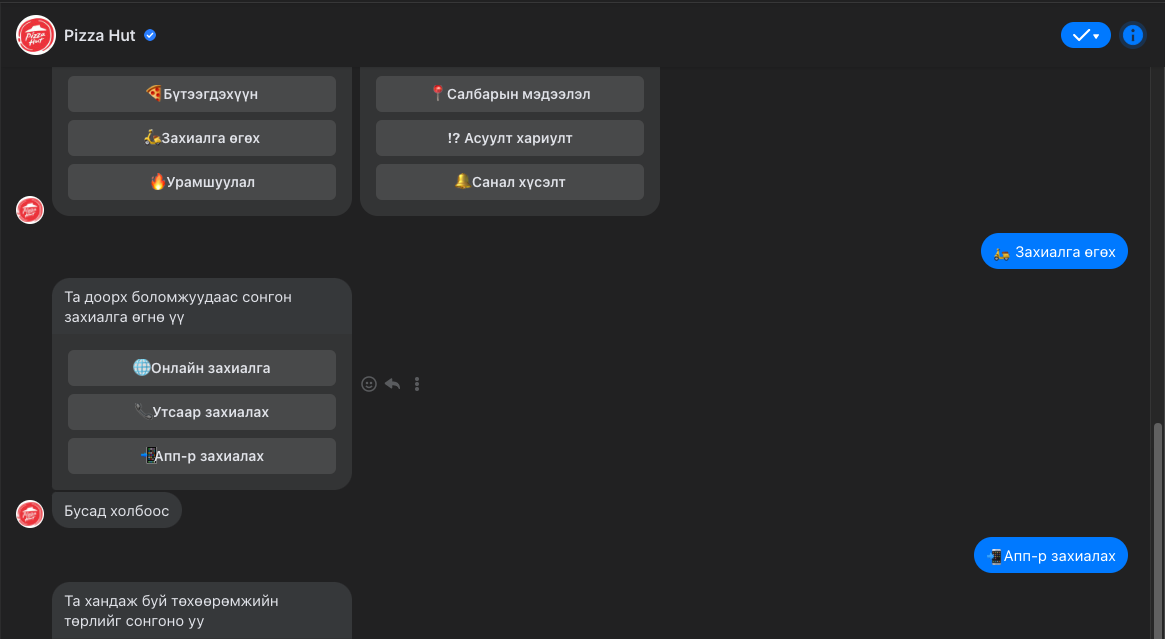
\includegraphics[width=\textwidth]{images/pizzaHut.png}
  \caption{Pizza Hut chat bot}\label{fig:chatbotPizzahut}
\end{figure}
\\Үйлчлүүлэгчдийн захиалга хүлээх хугацааг багасгахын тулд захиалгын үйл явцыг хурдасгаснаар тодорхой хэмжээнд нөлөөлж байгаа нь дээрх жишээнээс харагдаж байна.

\subsection{World Health Orgazination's Chat bot}
Цар тахал болох коронавирусын эрчимтэй тархаж байх үед дэлхийн өнцөг булан бүрд оршин суугаа хүмүүст цар тахлын мэдээлэл, урьдчилан сэргийлэх арга, баталгаатай эх сурвалжийн мэдээллээр хангах зорилготой чатбот юм.
Дэлхий нийтээр вакцинжуулалтын хөдөлгөөн өрнөж байх үеэр вакцины талаарх мэдээлэл, архаг хууч өвчинд нөлөөлөх талаар найдвартай, хамгийн сүүлийн үеийн албан ёсны мэдээллийг өгдөг. Хэдий халдварын тоо буурч, нийгэм өөрөө дасан зохицож байгаа хэдий ч Дэлхийн Эрүүл Мэндийн байгууллага үүргээ гүйцэтгэж чухал эх сурвалжаар хангасаар байгаагийн шинж юм. 
\begin{figure}[ht]
  \centering
  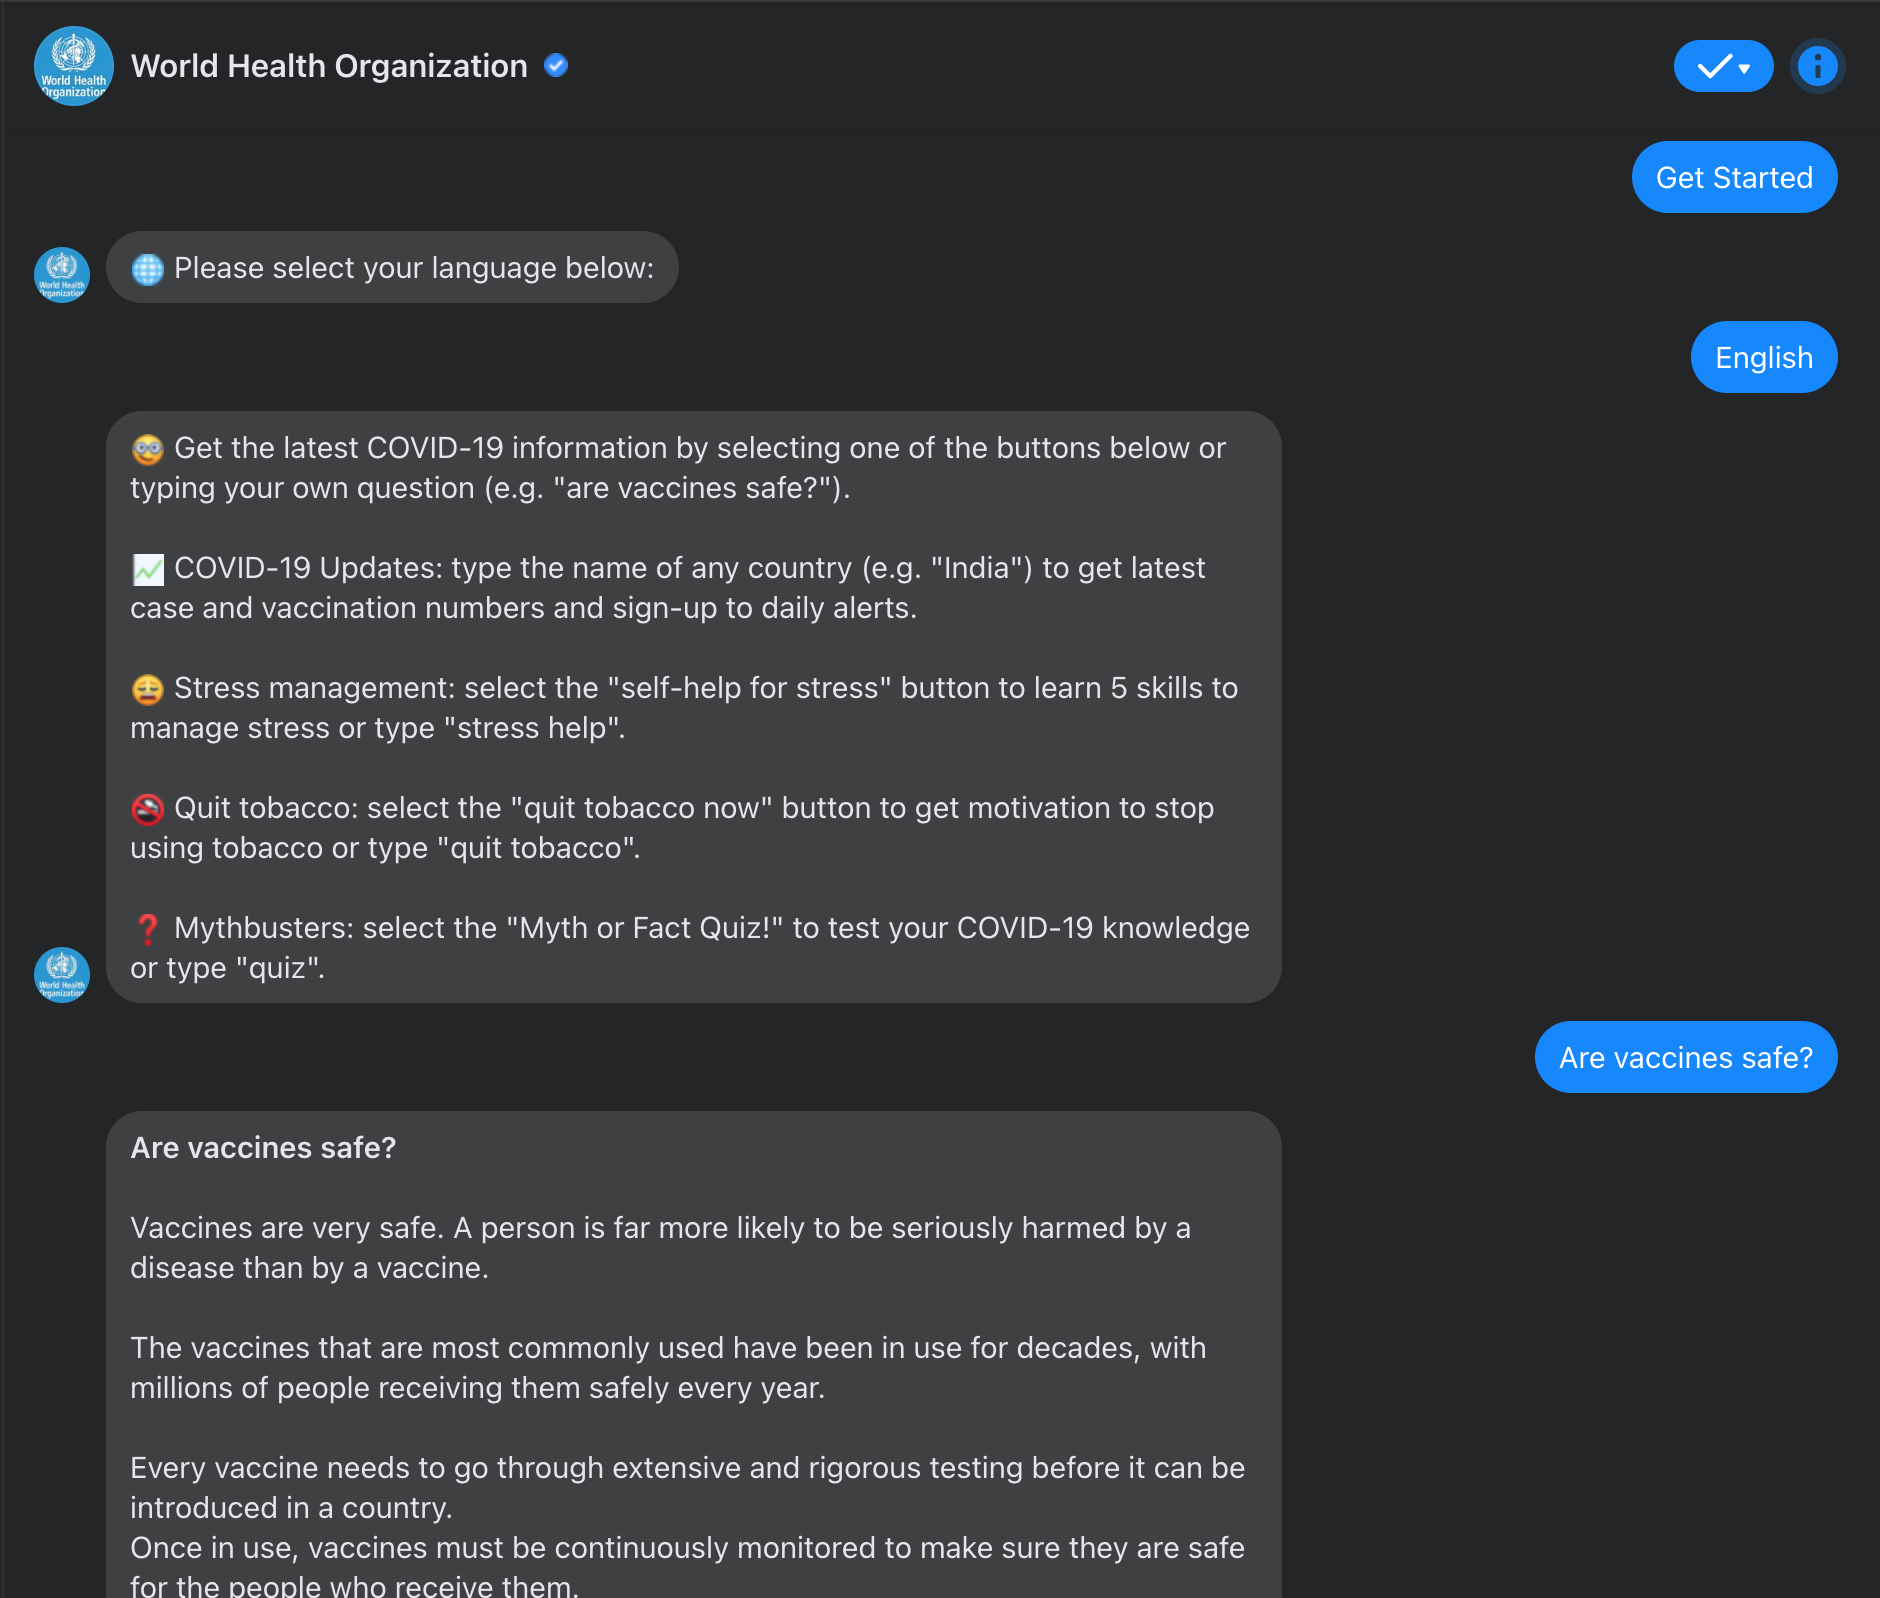
\includegraphics[width=\textwidth-4cm]{images/whoBOT.png}
  \caption{WHO's chat bot}\label{fig:chatbotWHO}
\end{figure}
\section{Ашиглах технологиуд}
\@title-ыг хөгжүүлэхдээ өгөгдөл цуглуулгыг \textit{python} хэлний сан болох \textit{BeautifulSoup} HTML өгөгдөл задлах технологийг ашигласан бөгөөд чатбот системийн үндсэн хөгжүүлэлтийг \textit{Microsoft Bot Framework}-ийн тусламжтайгаар \textit{javascript} хэл дээр хөгжүүлэлтийг хийж гүйцэтгэсэн. Чатбот болон өгөгдлийн сантай холбогдох буюу back-end хөгжүүлэлтийг \textit{node.js}-ийн framework болон \textit{express.js} ашигласан. Харин цуглуулсан өгөгдлийг AWS-EC2 сүлжээнд байршуулсан бөгөөд дүн шинжилгээ хийхдээ \textit{CSV} файлд хадгалан ашигласан.Ашигласан тенхологиудыг жагсаан бичвэл:
\begin{itemize}
  \item BeautifulSoup
  \item Amazon-Web-Services
  \item PostgreSQL
  \item SQLAlchemy - ORM
  \item Express.js
  \item Comma Separated Values - CSV файл
  \item Microsoft Bot Framework
\end{itemize}